\documentclass[conference]{IEEEtran}
\usepackage{amsmath,amssymb,booktabs,graphicx,microtype,cite,url,balance}
\usepackage{fontspec,xeCJK}
\usepackage[hidelinks]{hyperref}
\setmainfont{Times New Roman}
\setCJKmainfont{SimSun}
\XeTeXlinebreaklocale "zh"
\XeTeXlinebreakskip=0pt plus 1pt
\newcommand{\sisdr}{\mathrm{SI\text{-}SDR}}

\title{因果预测条件下的海洋声音分离 BS-RoFormer}
\author{\IEEEauthorblockN{匿名作者}\IEEEauthorblockA{匿名单位}}

\begin{document}
\maketitle

\begin{abstract}
本文检验：仅由此前海洋录音因果预测得到的背景频谱，能否帮助分离下一个 5 秒窗口中的声学事件。
FC-BSR 通过特征拼接、特征线性调制（FiLM）或交叉注意力把预测结果注入 BS-RoFormer。在包含
13 类信号的受控实验中，FiLM 在固定 0-dB 输入 SNR 下将 SI-SDR 改善量（SI-SDRi）提高
0.692 dB（95\% 配对 bootstrap 区间 $[0.542,0.847]$）。但在 42 小时连续真实水听器背景上，
条件收益取决于信号强度：$-18$ 与 $-12$ dB 时分别优于无条件模型 0.728 与 0.525 dB，在约
$-4$ dB 以上则转为落后。在没有隔离声轨的 1276 个真实鲸声事件上，FC-BSR 略微提高事件声轨
概率，却未降低残余事件概率或区间外改动。因此，预测先验在受控和弱目标场景中有用，但尚未证明
其能改善未知真实事件。
\end{abstract}

\begin{IEEEkeywords}
海洋声学，源分离，声景预测，BS-RoFormer，无参考评估
\end{IEEEkeywords}

\section{引言}
海洋背景随航运、天气、生物活动和季节变化\cite{miksisolds2013indian}。仅使用混合声音的分离器
必须从同一观测中同时推断突发事件与变化背景。本文改为使用此前声景提供严格因果先验：
\begin{equation}
 S_{t-H:t-1}\xrightarrow{P_\psi}\widehat S_t,\qquad
 x_t=N_t+\alpha s_t\xrightarrow{F_\phi(\cdot\mid\widehat S_t)}(\hat s_t,\hat N_t),
\end{equation}
其中分离器从不观察当前干净背景 $N_t$。

时域分离器\cite{luo2019convtasnet,luo2020dprnn}、注意力模型
\cite{subakan2021sepformer,wang2023tfgridnet}和子带系统
\cite{luo2023bsrnn,lu2023bsroformer}提供了强大的仅混合输入骨干。混合 Transformer 与 MixIT
扩展了架构和监督方式\cite{rouard2023htdemucs,wisdom2020mixit}，但没有检验下一时刻背景预测。
FiLM、交叉注意力与跨模态分离\cite{perez2018film,vaswani2017attention,zhao2018pixels}启发了三种
接口；递归、线性与分块预测模型则提供时间序列基线
\cite{salinas2020deepar,oreshkin2020nbeats,zeng2023dlinear,nie2023patchtst}。

本文贡献为：（1）FC-BSR，\footnote{代码与复现实验说明：
\url{https://github.com/D-eval/ocean_noise_pred_splite}。}以及严格匹配的拼接、FiLM 与交叉注意力
消融；（2）包含鲸声扫频和船噪过程的 13 类海洋感知信号生成器；（3）在 5 秒真实背景上比较
基线、oracle、预测和错时条件的信号强度扫描；（4）在未修改鲸声事件上直接比较 FC-BSR 与
BS-RoFormer。三级证据刻意分开合成真值与真实语义迁移。

\section{方法}
\subsection{背景预测与条件分离}
历史三分之一倍频程声级（TOL）$S_{t-H:t-1}\in\mathbb R^{H\times F}$ 只用训练集统计量归一化。
残差 GRU 预测
\begin{equation}
 z_t=\operatorname{LN}(\operatorname{GRU}(S_{t-H:t-1})),\quad
 \widehat S_t=S_{t-1}+g_\psi(z_t).
\end{equation}
零初始化精确表示 persistence；只有验证 MAE 优于 persistence 时才保留学习式预测
\cite{gneiting2011pointForecast}。

BS-RoFormer 将混合 STFT 映射为子带 token $X_k$。在轴向 Transformer 前的相同位置比较
\begin{align}
\text{拼接：}\widetilde X_k&=X_k+f([X_k;P_k(\widehat S_t)]),\nonumber\\
\text{FiLM：}\widetilde X_k&=(1+\tanh\gamma_k)\odot X_k+\beta_k,\label{eq:inject}\\
\text{交叉注意力：}\widetilde X&=X+\operatorname{Attn}(X,E(\widehat S_t),E(\widehat S_t)).\nonumber
\end{align}
所有残差条件分支均从恒等映射开始。损失结合波形 $L_1$ 与多分辨率复数 STFT；仅 TOL 代理实验
加入 $0.2\|\widehat S_t-S_t\|_1$。真实波形实验在训练分离器前冻结预测器。

\begin{figure*}[t]
\centering
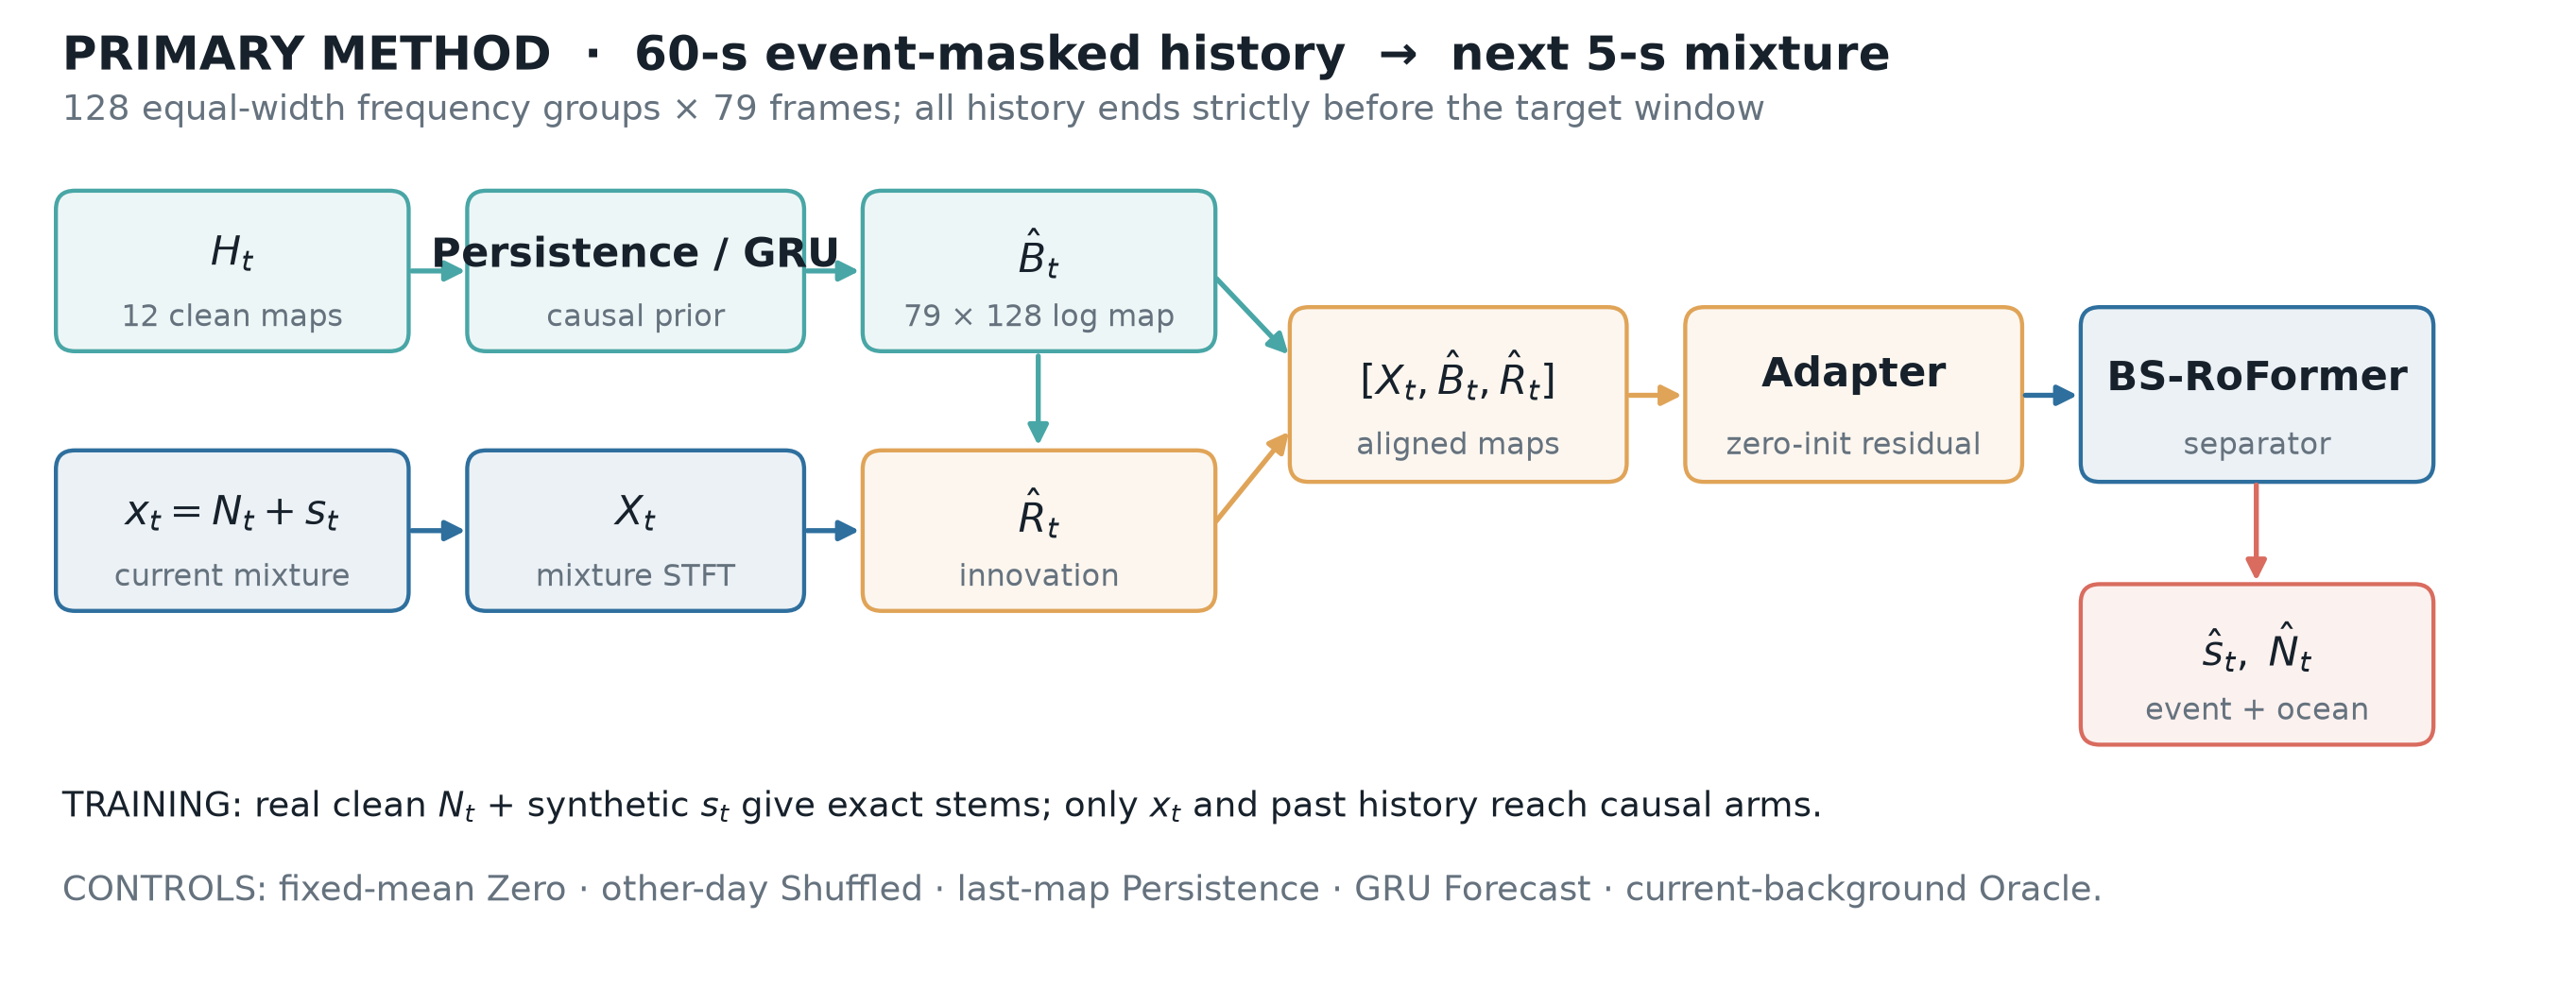
\includegraphics[width=.94\textwidth]{figures/architecture.png}
\caption{FC-BSR 架构。严格早于当前时刻的声景特征预测当前背景频谱，并条件化同一个
BS-RoFormer 骨干；移除蓝色路径即得到参数匹配的无条件基线。}
\label{fig:architecture}
\end{figure*}

\subsection{海洋感知合成信号分布}
生成器包含 13 类：谐波、线性啁啾、非谐波、脉冲列、调频音、带限噪声、鲸声上扫、下扫、拱形、
S 形、脉冲包、船舶音调和船舶空化。鲸声代理由 1--3 个局部事件组成，随机改变时长、曲率、
分音、渐入渐出与抖动。船舶音调和窄带空化分量以 0.8 概率采用 5--20 Hz 低频振荡器（LFO）
音量包络；宽带分量不做该调制。训练 SNR 在 $[-12,12]$ dB 均匀抽样。这些代理用于覆盖轮廓和
调制样式，并不声称对应具体物种。

频谱位移同时用方向性 $D_{\rm KL}(p\|q)$ 和有限对称 JS 散度\cite{lin1991divergence}衡量，
另报告频谱熵与信号--海洋频谱重叠。更大的 KL/JS 只代表覆盖范围更广，不等价于语义多样性。

\subsection{证据层级与实验协议}
第一层使用 NOAA--Navy SanctSound 小时级 TOL 产品\cite{noaa2020sanctsound}。MB03 部署
01--02/03/04 分别作为训练/验证/测试集。随机相位逆变换只产生受控频谱代理，不能称为恢复音频。
所有波形为 5 秒；每个训练部署使用 4000 个样本，共训练 2500 步。

第二层使用 42 小时连续 8-kHz 水听器 WAV，其中 12/6/24 小时用于训练/验证/测试。当前真实
干净波形 $N_t$ 与合成目标直接混合。主实验使用 5 秒混合、2500 步训练，并在 $-18$ 至 $+12$
dB 的 11 档 SNR 上测试。单独的预测分辨率诊断固定一小时历史，将步长设为 5 秒、30 秒、1 分钟
或 10 分钟；其后的实验全部恢复为 5 秒波形。

第三层使用按日期隔离的 2-kHz DCLDE 2013 露脊鲸录音\cite{gillespie2019dclde}。事件标注可
支持检测\cite{shiu2020marine}，但不存在隔离声轨。仅向标注干净的训练片段注入上述代理，测试
1276 个未修改的真实阳性事件。两种模型共享样本、种子、骨干初始化、2500 步预算和仅验证集选点。

前两层使用尺度不变投影的 SI-SDR 与 SI-SDRi\cite{vincent2006sdr,leroux2019sdr}。全部不确定性
区间来自固定种子的配对 bootstrap；连续片段按录音小时分块，真实事件按留出日期分块。当前测试
频谱只可用于监督或 oracle 对照，因果历史严格截止于 $t$ 之前。

\section{实验与结果}
\subsection{条件机制选择与信号多样性}
表\ref{tab:ablation}只按验证集选择 FiLM。在 832 个固定 0-dB 配对样本（每族 64 个）上，
它将 SI-SDRi 从 4.850 提高到 5.541 dB。逐频带缩放与偏置可以直接表达“此处为预期能量”；
拼接需要压缩加倍特征，交叉注意力则必须在相同预算内从粗条件中学习对齐。

\begin{table}[t]
\caption{匹配的 5 秒条件注入消融（dB）。}
\label{tab:ablation}\centering\footnotesize
\begin{tabular}{lrrr}
\toprule
注入方式 & 验证 SI-SDRi & 测试 SI-SDRi & 配对 $\Delta_0$\\
\midrule
无条件 &4.864&4.059&0\\
拼接 &5.343&4.432&+0.623\\
FiLM &\textbf{5.419}&\textbf{4.468}&\textbf{+0.692}\\
交叉注意力 &5.128&4.261&+0.331\\
\bottomrule
\end{tabular}
\end{table}

FiLM 在五类鲸声代理上的增益依次为 0.869、0.835、0.919、0.906 与 0.806 dB。船舶音调最难：
尽管相对增益为 0.320 dB，条件模型的绝对 SI-SDRi 仍为 $-8.295$ dB。总体增益与 JS 的相关性
很弱（$r=-.057$），与频谱熵也仅为 $r=.122$；因此提高散度能扩大覆盖，却不能预测先验何时有用。

\subsection{真实背景：时间尺度与目标强度}
表\ref{tab:windows}的分辨率诊断对各模型使用相同留出样本。只有 5 秒预测器在验证集优于
persistence（MAE 1.366 对 1.386 dB）；其他尺度均选择 persistence。四种条件分离器均优于
匹配基线，但区间彼此重叠，故不能据此判定最佳时间尺度。

\begin{table}[t]
\caption{真实背景上的预测分辨率诊断。}
\label{tab:windows}\centering\footnotesize
\begin{tabular}{lrrrr}
\toprule
步长 & 预测器 & 条件模型 & 基线 & 增益 [95\% 区间]\\
\midrule
5 秒 &GRU&29.753&28.527&1.226 [1.082,1.381]\\
30 秒&persistence&29.630&28.534&1.095 [0.935,1.265]\\
1 分钟&persistence&29.661&28.533&1.128 [0.971,1.298]\\
10 分钟&persistence&29.711&28.535&1.176 [1.036,1.326]\\
\bottomrule
\multicolumn{5}{l}{\scriptsize 条件模型、基线与增益均为目标 SI-SDRi（dB）。}
\end{tabular}
\end{table}

更困难的固定 5 秒实验在 1152 个配对测试混合上比较 BS-RoFormer、当前真值频谱 oracle、因果
预测和错时条件。跨训练 SNR 平均后，基线为 23.470 dB，Forecast-FC-BSR 为 22.871 dB
（$\Delta=-0.599$，区间 $[-0.851,-0.346]$），oracle 平均值也更低。这暴露了简单分辨率诊断
没有显示的条件化/容量影响。图\ref{fig:strength}进一步表明：在 $-18,-15,-12,-9,-6$ dB，
预测条件分别提高 0.728、0.643、0.525、0.366、0.157 dB；从 $-3$ dB 开始转为落后。错时条件
对最弱目标也有收益，却随 SNR 上升迅速退化，因此不能把弱目标增益完全归因于预测的时间准确性；
正则化或额外容量仍是可能解释。

\begin{figure}[t]
\centering
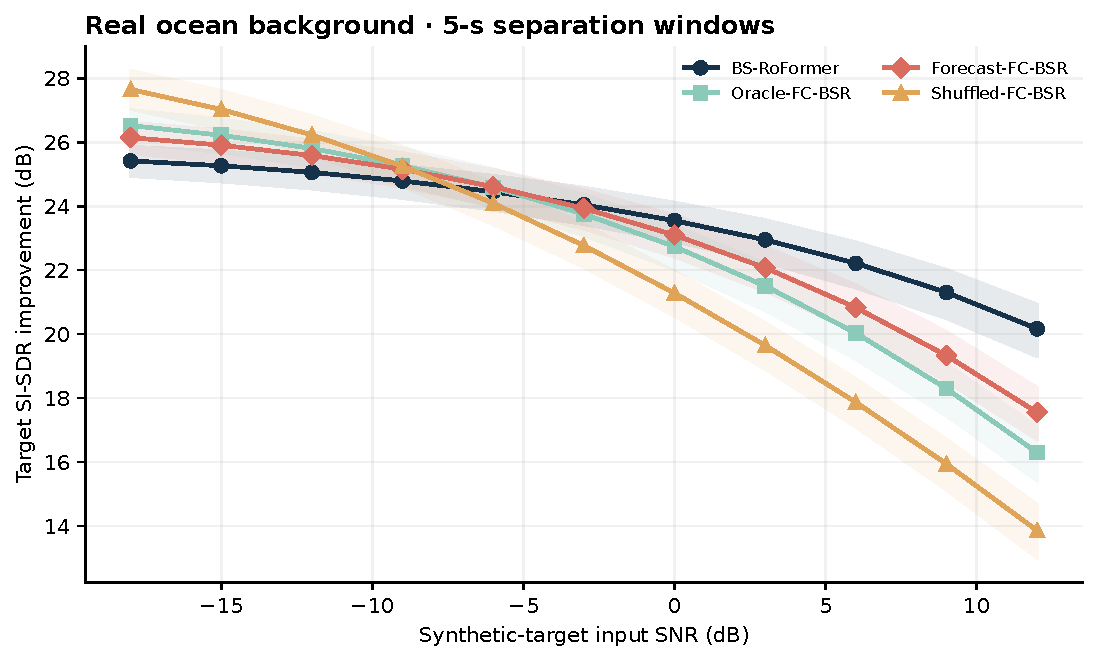
\includegraphics[width=\columnwidth]{figures/real_strength_sweep.pdf}
\caption{5 秒真实海洋背景上的目标强度扫描。四条曲线对应全部模型条件，阴影为配对 95\% 区间。}
\label{fig:strength}
\end{figure}

\begin{figure*}[t]
\centering
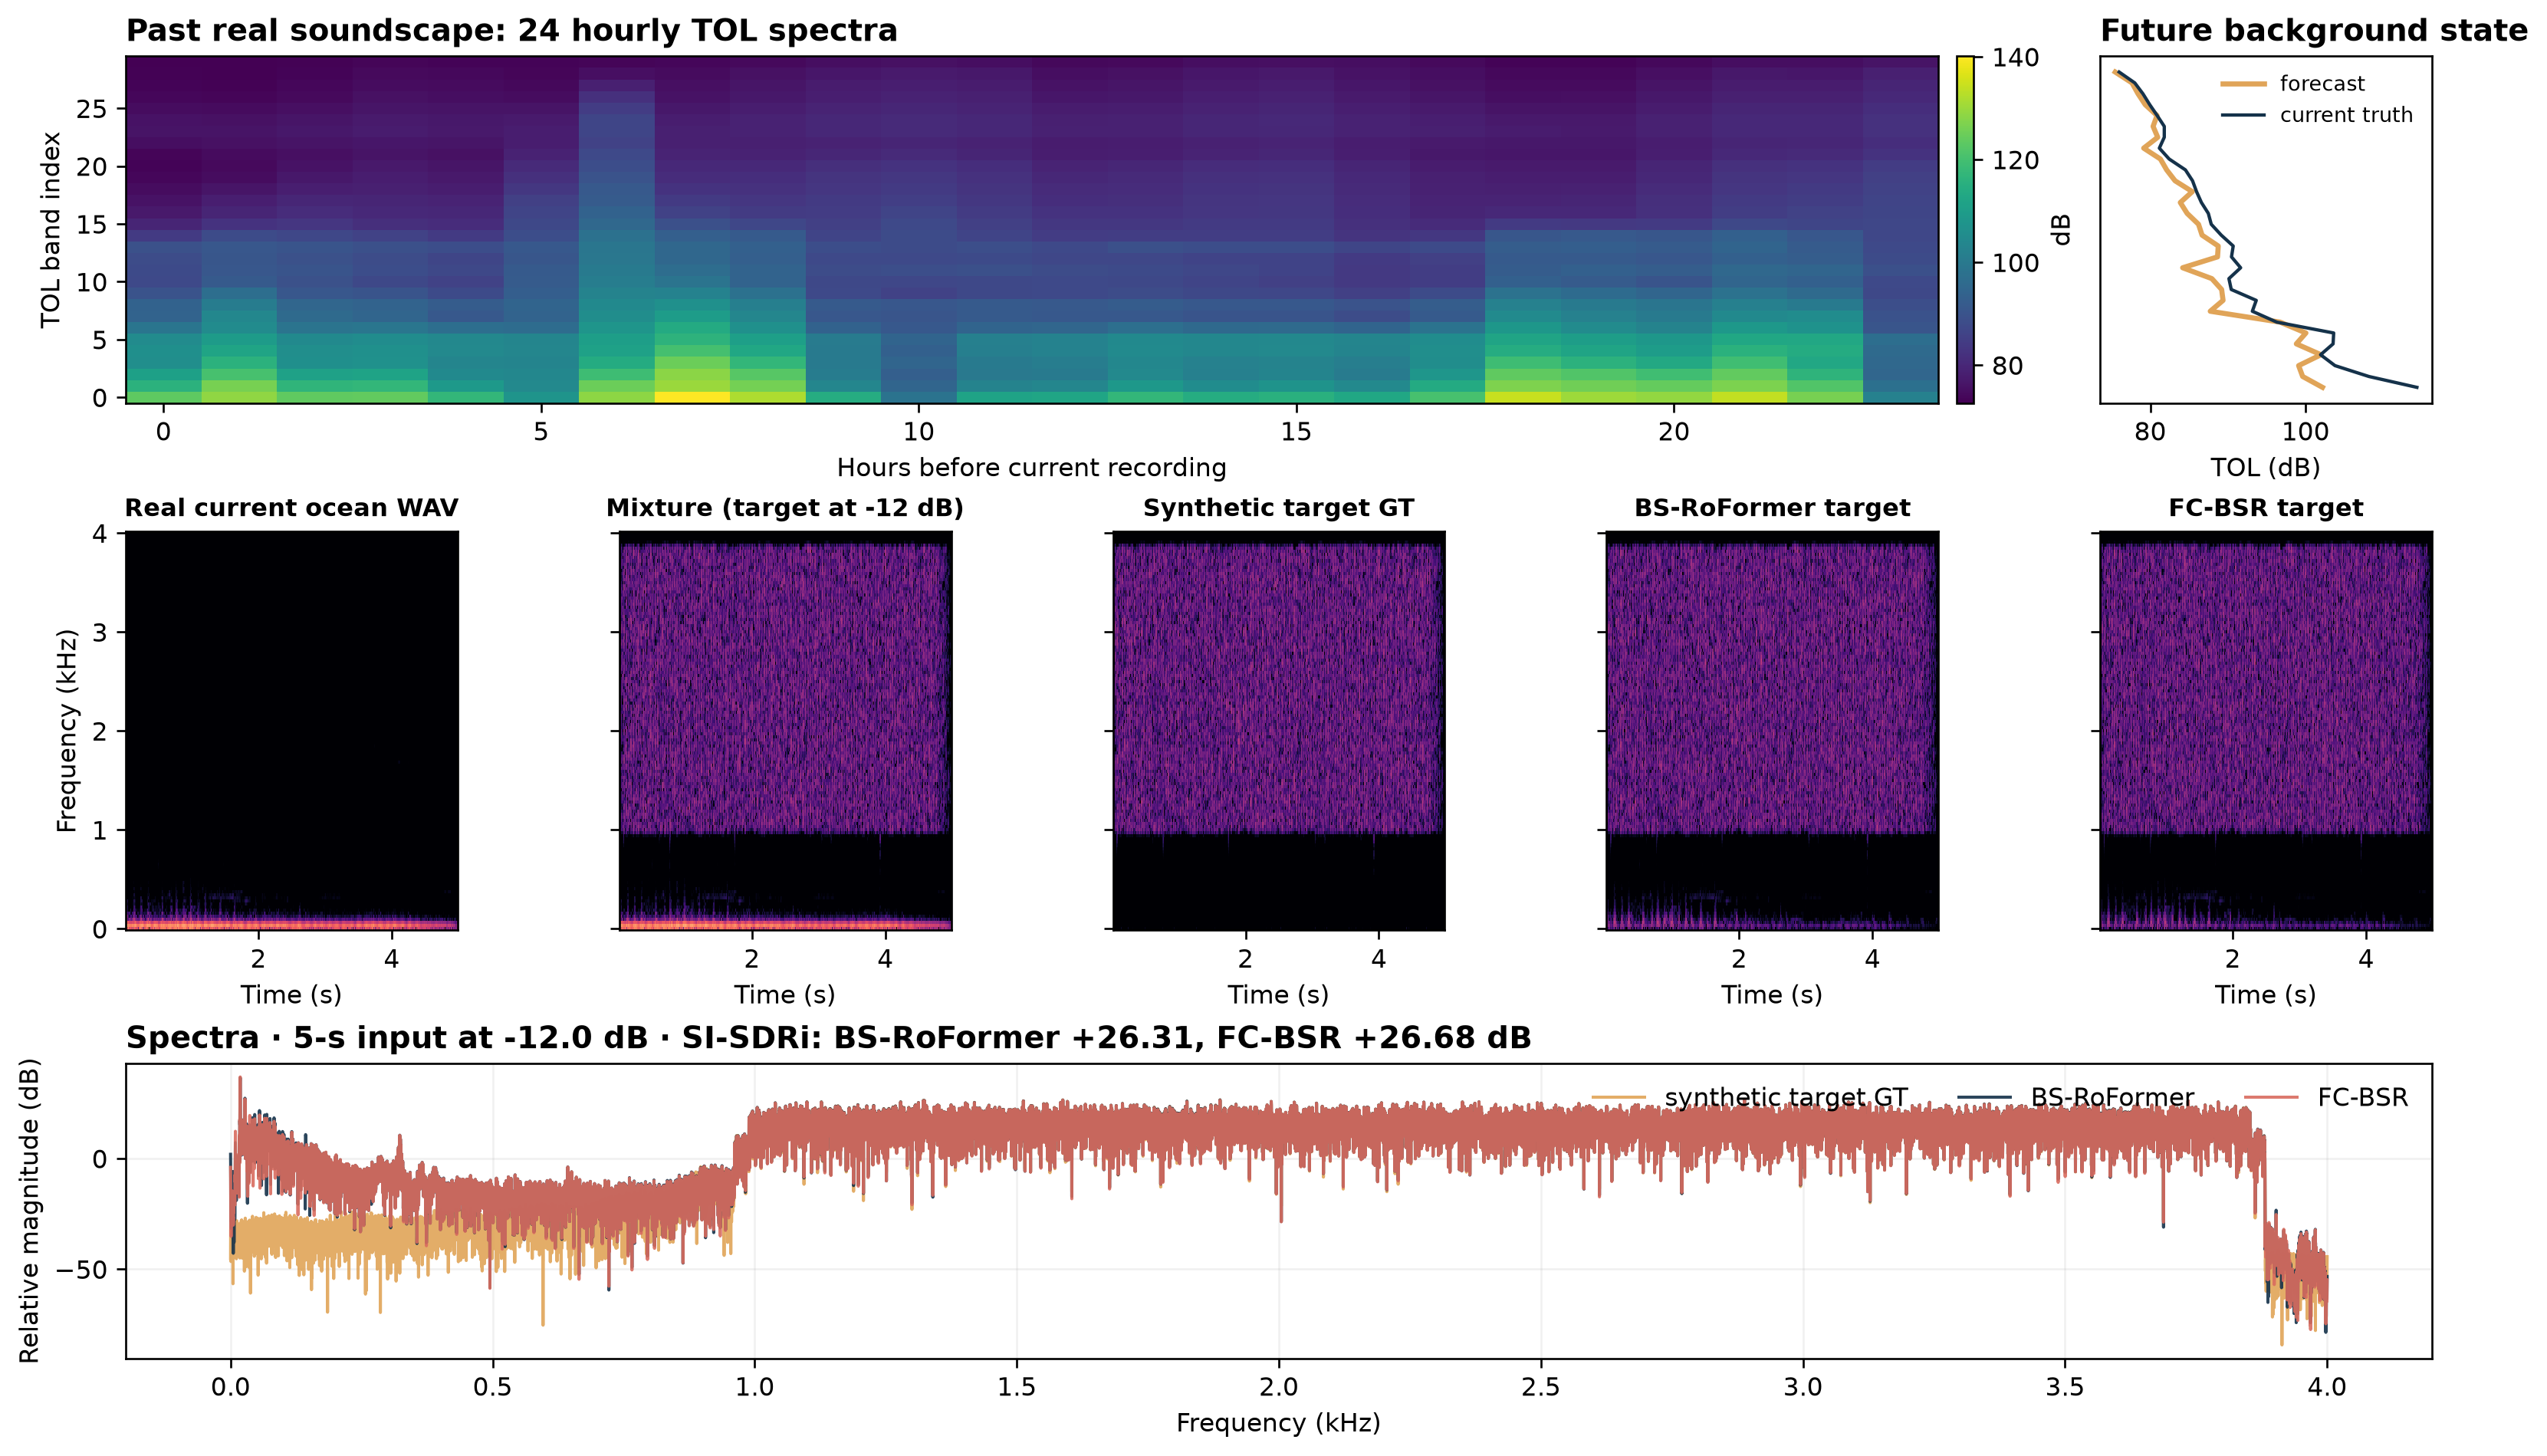
\includegraphics[width=.98\textwidth]{figures/real_audio_visualization.png}
\caption{真实海洋背景中的一个代表性弱目标（$-12$ dB，5 秒）。该示例避免目标在视觉上压倒背景，
并把 BS-RoFormer、FC-BSR 与精确目标并排比较。}
\label{fig:example}
\end{figure*}

\subsection{没有分离真值的真实事件}
参考学习式无参考指标\cite{kilgour2019fad,grais2019referenceless}和语义音频嵌入
\cite{wu2023clap,xiao2024clapscore}，我们训练、校准并冻结二分类器；测试 AUROC、AP 与 F1
分别为 .9723、.9755、.9275。混合一致性要求 $\hat N=x-\hat s$。将 $\hat s$ 按
$\{-60,-30,-24,-18,-12,-6,0\}$ dB 逐级恢复，检查事件概率是否单调回升；Identity 与
all-to-event 排除平凡解，标注区间外变化审计背景保留。

12 个 5 秒历史窗的预测器把验证 MAE 从 2.076 降到 1.974 dB，随后冻结。在代理验证集上，
BS-RoFormer 与 FC-BSR 的 SI-SDRi 为 11.125 与 11.088 dB。表\ref{tab:events}给出未修改真实
事件结果。FC-BSR 的事件声轨概率略高（$+.0051$），但残余事件概率更高、单调率不变，且区间外
改动增加；残余概率差 $+.0145$ 的日期分块区间为 $[-.0177,.0269]$。因此这一层证明分离器能
迁移到真实事件，但没有证明预测条件优于无条件模型。

\begin{table}[t]
\caption{1276 个真实事件上的匹配比较。}
\label{tab:events}\centering\footnotesize
\begin{tabular}{lrrrr}
\toprule
方法 &$p(\hat N)\downarrow$&$p(\hat s)\uparrow$&单调率$\uparrow$&区间外$\downarrow$\\
\midrule
BS-RoFormer&\textbf{.751}&.863&\textbf{.940}&\textbf{.279}\\
FC-BSR&.766&\textbf{.868}&.939&.288\\
\bottomrule
\end{tabular}
\end{table}

\begin{figure}[t]
\centering
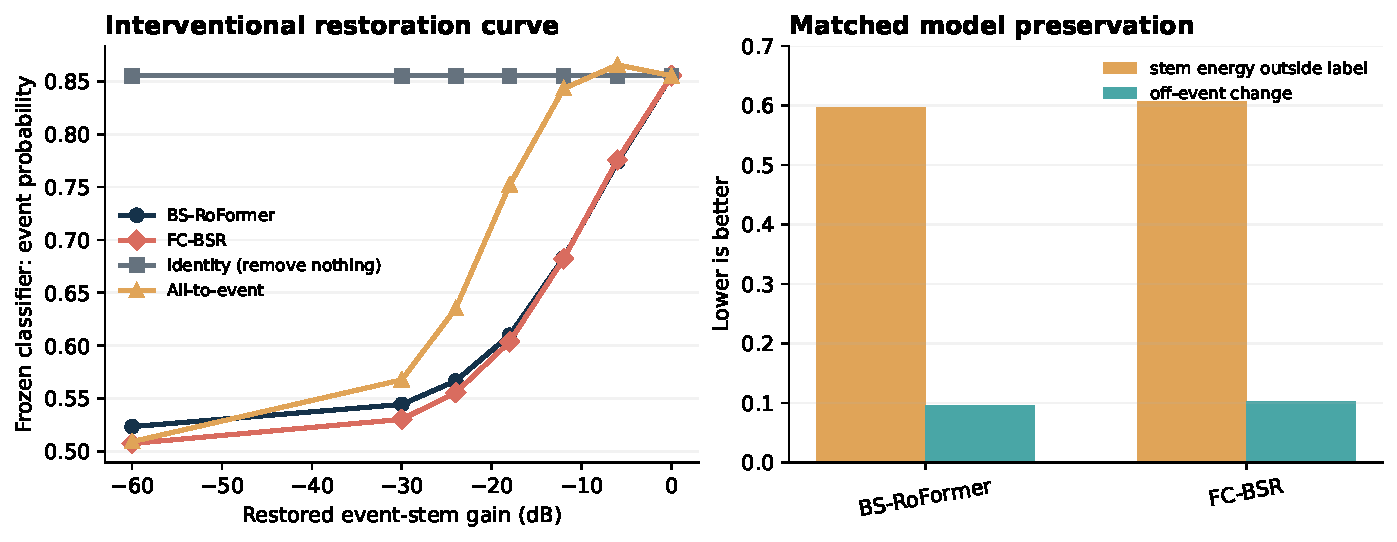
\includegraphics[width=\columnwidth]{figures/dclde_reference_free.pdf}
\caption{无参考恢复曲线与背景保留审计。两种模型都进行了非平凡语义分离，但 FC-BSR 在真实事件上
没有全面胜出。}
\label{fig:real}
\end{figure}

\section{讨论与结论}
证据支持的结论比初始假设更窄：FiLM 是受控真值下最佳的条件接口；在 5 秒真实背景中，先验有助于
弱目标。但其收益并不普遍：信号增强后增益反转，oracle 也未改善平均值，且未修改鲸声上没有显示
预测条件优势。四种预测分辨率中还有三种由 persistence 获胜。这些负对照很关键：它们区分了
“背景信息存在价值”与“当前架构总能利用该信息”。

系统已适合实验检查：真实波形模型的 RTF 约为 .0028，本地前端可显示预测并试听、下载两条估计
声轨，但这不等于野外部署。后续应根据预测不确定性选择性启用条件，覆盖多站点、多季节，并为真实
事件获取隔离声轨或更强局部参考。分类器恢复曲线是语义迁移证据，不能替代波形保真真值。

\clearpage
\balance
\bibliographystyle{IEEEtran}
\bibliography{reference}
\end{document}
